\chapter{Related work}

I will use this chapter as an insight into the world of agents and spatial memory. I hope that you will not be disappointed, since there is no 007 in following lines.

\section{Agents}

There are several ways how to explain what or who the agent is. Apart from systems of agents used in philosophy or sociology, we can see a first modern use of agency and agents in economy where economists have substited the human with a simpler agent. They intended to simplify their economic models to be able to actually simulate something. Buyers and sellers are typical examples of agents used in simplified market model in microeconomics (see []). In this context agents are entities in the model which can act based on situation in the model.

For area of artificial intelligence we can use the definition of an agent which can be found in \cite{russel2003ai}. It cannot be more simple:

\begin{definition}{\bf Agent} is just something that acts.
\end{definition} 

Of course it is as general as it could be and for my purposes it is too simple, so I will use another definition which meets better the context of my work.

\begin{definition}{\bf Agent} is something that senses the environment and affects it using its actuators.
\end{definition} 

Having that defined we continue to specific kinds of agent. In this thesis I use several slightly varying terms about agents: {\emph rational, autonomous, plausible and believable}. 

A rational agent refers back to economics where we can find a definition of rational behaviour. Even though it is rather a hypothetical model, as people are usually irrational in their decisions from the economics perspective, their is yet nice definition whereby a rational agent acts as if balancing costs against benefits to arrive at action that maximizes personal advantage (Milton Friedman (1953), Essays in Positive Economics). So simply he does what is or perhaps might be best for him based on his current knowledge of the world.
 
On the other hand, the rational behaviour might be understood in a completely different way. Plausible agents are such agents, where the basic approach is to implement human-like internal processes. One of the well-known example is neural networks, although they are usually used in quite simplified way. Since it is really difficult to implement completely plausible agent, one can see research teams focusing on a specific part of the complex human being. 

Autonomous agents are those agents which are capable of accomplishing useful tasks or are effective problem solvers \cite{Loyall:believableagents}. A

Believable agents are personality-rich autonomous agents with the powerful properties of characters from the arts \cite{Loyall:believableagents}. Now there is just the autonomous agent left. An autonomous agent should be able to accomplish useful task or be an effective problem solver. I would like to add one more term which is going to fit the agents I use. 

Belief-Desire-Intention (BDI) agency model implements the three parts agent's belief, desire and intention and use them when comes to reasoning. A BDI agent is particular part of bounded rational agent who use those three parts to separatly prepare plans which are later executed. What a BDI distinguishes from a simple reactive agent is a reactive agent creates immediate decisions based on current state of environment and inputs of his sensors. On the other hand, a BDI agent uses the three parts:

\begin{itemize}
\item {\bf belief} represents the agent's informational state, for example sensory inputs and information in his memory,
\item {\bf desire} is the agent's motivational state, what he needs to approach, for example he is hungry and he needs to find appropriate food,
\item {\bf intention}, on the other hand, is his immediate decision how he attaing the goal he desires, in other words it is execution of plan, for example next move.
\end{itemize}

\section{Spatial resource-bounded memory}

A memory is something what changes a reactive agent into an agent with ability to learn. It can be used for learing consequances of agent's acts, conditional dependencies in the agent's world (citation for bayesian networks), or spatial information about the environment. The latter one is a kind of memory I used for agents in my simulation. 

A spatial memory is used when agent needs to navigate in usually two or three dimensional space. In short it is a component of an agent which says him where to go when he needs or want to do something. There are several different approaches and a couple of examples are going to be covered in this section. I am going to introduce several existing implementations of spatial memory. Mainly I will focus on if and how they have dealt with bounded resources - either due to implementation restrictions, or when approaching plausibility in their models. 

\subsection{Resource-bounded reasoning}

Rational agents cannot be expected to be able to compute a load of data in a constant time or in a time in which the environment doesn't change much. That is why we have to take into account bounded resources when simulating plausible or rather real agents. What we want to avoid here is the computation of plan takes a long period of time during which the environment changes significantly. As they have mentioned in \cite{Bratman:practicalreasoning}, we could separate plan computation from execting the plan, whereby the plan is prepaired over several executions. In that case we need either to be able to perfectly predict the future, or base our plan on data which does not change at all or is frozen for the given period of time.

\subsection{Short-term and long-term memories}

Generally, when I talk about remembering something, I should mention two terms: a long-term memory (LTM) and a short-term memory (STM). Both of which describes a capacity for holding certain amount of information in mind. Apart from the varying amount, the memories differ in availability of such information and a period of time the memories last.       

In 1968 Richard Atkinson and Richard Shiffrin suggested in \cite{Atkinson:humanmemory} a memory model parted into three components: 

\begin{enumerate}[(a)]
\item sensory register being able to store only a relatively small amount of data for a short period of time,
\item short-term store with ability to store also limited amount of data, but for quite a longer period of time,
\item long-term store with a huge capacity for nearly unlimited time.
\end{enumerate}

\begin{figure}
  \centering                                
  \includegraphics[scale=0.5]{diagrams/usedalgorithms/atkinson-memory.eps}    
  \caption{Information flow in the memory system has been depicted in \cite{Atkinson:controlofrtm}.}
  \label{usedalgorithms:qttv}
\end{figure}

We use the {\bf short-term memory} for storing pieces of information for relatively short period of time. That could be seconds or minutes. A number of entites we are able to hold in our STM was researched by George Miller in 1956 as it is mentioned in \cite{Sternberg:congitivepsychology}. The outcome of his work was the magical number 7+-2, which is the number of similar small things we can remember in STM.

A long-term memory, on the other hand, is used for information we do not think of consciously, but but pieces of such information are important for our everyday life. The capacity of LTM memory is unknown, as there is no way how to find it. 
                                               
\subsection{Computational memory architectures}

Computational memory architectures for autobiographic agents interacting in complex virtual environment suggested by Ho in \cite{Ho:memoryarchitectures}. works with both short-term and long-term autobigraphic memory, where they have observed agent’s ability to survive comparing to purely reactive agency model. Moreover, they researched whether the narrative communication amongst agents somehow positively influence those agents. They have separately experimented with three types of agents: purely reactive (PR), short-term memory (STM) and long-term memory (LTM). Purely reactive agent walks randomly around the environment avoiding obstacles and searching for resource objects to fulfill his needs. What a pure reactivity means is the agent moves randomly until an event occurred such as a collision with obstacle or a resource object detection.

STM agents in \cite{Ho:memoryarchitectures} further extend the model of purely reactive agents and add a Track-back memory system in addition to the reactive behaviour. Each time an agent deals with an event (e.g. collision, or resource object) he puts such information into his memory. They refer to this as an event-based memory entry making mode. Those events are kept in a linear list of a finite size, whereby the oldest events are cut off. The memory is used when an internal variable is over threshold. That is the moment when agent searches in his memory for an information about relevant resource object. If he succeeded, he retrospectively undoes all memorized states leading to the relevant one. So, what they actually store in memory is an agent’s current state: where he was and what he perceived. While attaining imperfection in retrieving information from short-term memory, they introduced noise distortion using Gaussians.

Long-term memory model is mostly based on psychological autobiographic memory models. There are three parts that are involved in the reasoning process: Event specific knowledge (ESK), Event reconstruction process (ER) and Event filtering and ranking process.

\subsection{How Place and Objects Combine?}

This paper written by Brom et al \cite{Brom:placeandobjects} is mainly focused on plausible behaviour while searching things in structured spaces such as flats. Apart from others who previously researched the area of spatial memory for plausible agents, they suggested a model for an agent which could successfully live in a dynamic environment with objects which could be moved without the agent’s involvement. 

In this model the environment consists of abstract and concrete areas such as rooms and pieces of furniture respectively. Those areas are combined into a tree structure used in the model where e.g. the flat is a root node, the immediate child nodes are rooms and, finally, concrete pieces of furniture are child nodes below room nodes. They have created four different categories for objects to reflect varying probabilities of changing object’s location which fact simulates a presence of another agent in the environment. So the observed agent does not leave the flat and he is alone there.

During their experiments, what is interesting for my work is they subsequently observed the ability of the model to emerge the searching rules from scratch, to relearn the rules in case of changing particular settings, and if the merged rules meet with the human behaviour, i.e. they are believable. 
                 
\subsection{Inspirations for my work}

The suggested RTM and LTM models of agents in \cite{Ho:memoryarchitectures} are more than interesting to be implemented in my simulation. There has to be a couple of minor changes, though, as I am working with a simpler environment comparing to the one used in the work described above. The changes will influence the structure of memory records in both RTM and LTM. Also the communication protocol will be different and I am going to introduce it later in this thesis. Although it is not going to be part of this particular thesis, having compared their memory models is defenitely promising.

In my project the environment I want to use doesn’t have differentiated area as is in \cite{Brom:placeandobjects}, that means it is homogeneous. For the purpose of implementing an agent with a simiral spatial "What-where" memory model, I will use different spatial organization which could be similarly structured into a grid.  The suggested model, however, is usable for objects which are moved around the environment and I don’t have such objects. Objects in my environment are generated around distribution place and locations of those places are something what could be learnt using “What-Where” model. 